% main-en.tex, English version. The Portuguese version is in main.tex.
\documentclass[11pt,a4paper]{article}

\usepackage[utf8]{inputenc}
\usepackage[T1]{fontenc}
\usepackage[english]{babel}
\usepackage{lmodern}
\usepackage{microtype}
\usepackage{geometry}
\usepackage{booktabs}
\usepackage{tabularx}
\usepackage{array}
\usepackage{graphicx}
\graphicspath{{figures/}}
\usepackage{hyperref}
\usepackage{enumitem}

\geometry{margin=2.5cm}

\hypersetup{
  colorlinks=true,
  linkcolor=blue,
  citecolor=blue,
  urlcolor=blue
}

\newcolumntype{Y}{>{\raggedright\arraybackslash}X}

\title{From Prompt to Process: A Systematic Review of AI-Assisted Software Development Frameworks}
\author{Sanderson Oliveira de Macedo\\
\textit{Federal Institute of Goias}\\
\texttt{sanderson.macedo@ifg.edu.br}}
\date{\today}

\begin{document}

\maketitle

\begin{abstract}
AI-assisted software development is no longer a matter of isolated prompts. It has reorganized itself around frameworks that structure the work with persistent artifacts, agentic roles, integrated execution, and validation. What has been missing is a review that takes these operational frameworks as its object, through a software engineering lens, rather than treating agent architectures in the abstract or cataloguing techniques tied to single lifecycle tasks. This article presents a systematic literature review conducted under the Kitchenham protocol. The review gathered 37 studies published between 2022 and 2026 after two screening passes and three rounds of snowballing, including only academic papers and archived preprints with verifiable records. A hybrid thematic synthesis derived six inductive themes and tested them against a proposed taxonomy of six dimensions: specification, context, roles, execution, validation, and portability. The evidence supports the shift from prompt to process, which holds in 34 of the 37 studies, and confirms five of the six dimensions. Portability is the weak one, surfacing almost always as a diagnostic risk rather than a design property, and two axes emerge outside the taxonomy: human-AI collaboration and security. We identify three recurring axes of tension and show that context and traceability, not code generation itself, are the field's transversal bottlenecks. We close with a process-oriented research agenda built around benchmarks that evaluate the pipeline, head-to-head comparison between frameworks, and longitudinal evaluation of governance.
\end{abstract}

\noindent\textbf{Keywords:} AI-assisted software development; AI agents; systematic review; software engineering; agentic frameworks.

\section{Introduction}

Language-model programming changed in nature within a few years. What began as code suggestions drawn from isolated prompts grew into systems that split the development cycle across specialized agents, keep persistent artifacts, run tools, and validate their own work. ChatDev and MetaGPT showed that organizing agents around engineering roles, rather than merely improving the prompt, changes what a system can deliver \cite{ChenQian2023,SiruiHong2023}. The more recent literature already speaks of AI-native software engineering and treats multi-agent systems as a research line in their own right \cite{hou2024llmse,AhmedEHassan2024,JundaHe2025}. The unit of work, once the prompt, has become the process.

This shift brings a new object of study: the operational framework that organizes development on top of an agent. Characterizing it means examining the function of each mechanism, how the specification drives generation, how repository context is retrieved, how roles are distributed, how execution acts on the environment, and how validation anchors the result, instead of surface metrics such as command counts or popularity. Existing reviews approach the problem from a different angle. Some classify agent architectures abstractly, by cognitive component; others map language-model techniques across isolated lifecycle tasks. What is absent is a software engineering lens trained on the frameworks that organize the development cycle at the level of process and repository, and a confrontation of their structure with the available evidence rather than a study-by-study description.

To fill that gap, we conducted a systematic literature review under the Kitchenham protocol, restricted to academic papers and archived preprints with verifiable records \cite{kitchenham2009slr}. From a final corpus of 37 studies published between 2022 and 2026, we propose a six-dimension taxonomy for classifying these frameworks and validate it empirically against the corpus through a hybrid thematic synthesis. The article makes three contributions: a six-dimension taxonomy (specification, context, roles, execution, validation, and portability) tested against the evidence rather than assumed a priori; a thematic synthesis of six inductive themes that covers 100\% of the corpus and exposes three axes of tension and two emergent axes outside the taxonomy; and a process-oriented research agenda that follows directly from the observed gaps.

The review is guided by five research questions. RQ1: which architectural dimensions distinguish these frameworks? RQ2: how do they organize context, roles, artifacts, execution, and validation? RQ3: what kinds of evidence support their claims? RQ4: which risks and limitations are reported or inferable? RQ5: which research gaps remain for comparing, evaluating, and governing these frameworks in real projects? The rest of the article is organized as follows. The Review Method describes the protocol and the selection flow; Related Work positions the review against the existing literature; the Proposed Taxonomy presents the six dimensions; Results and Synthesis consolidate the six themes and validate the taxonomy; the Discussion lays out the transversal findings and the axes of tension; and the Research Agenda and Conclusion outline the next steps.

\section{Review Method}

The Introduction framed AI-assisted development frameworks as a layer that organizes the work of whoever uses a development agent, and argued that comparing them requires examining the function of each mechanism rather than surface metrics such as command counts or popularity. We investigated this object through a systematic literature review (SLR) conducted under the Kitchenham protocol \cite{kitchenham2009slr}. The review covers only academic literature, that is, peer-reviewed papers and archived preprints with verifiable bibliographic records; sources without a citable paper were out of scope by construction. The cutoff date was May 26, 2026, and the coverage window ran from 2018 to 2026.

The protocol was fixed before execution and defines the research questions, the sources consulted, the inclusion and exclusion criteria, the extraction schema, and the snowballing strategy. The corpus grounds the analytical dimensions of the taxonomy and establishes the state of knowledge on agents, specification, validation, and risk. Figure~\ref{fig:metodologia} summarizes the review flow, from identification to reporting, with the real counts at each step.

\begin{figure}[h!]
\centering
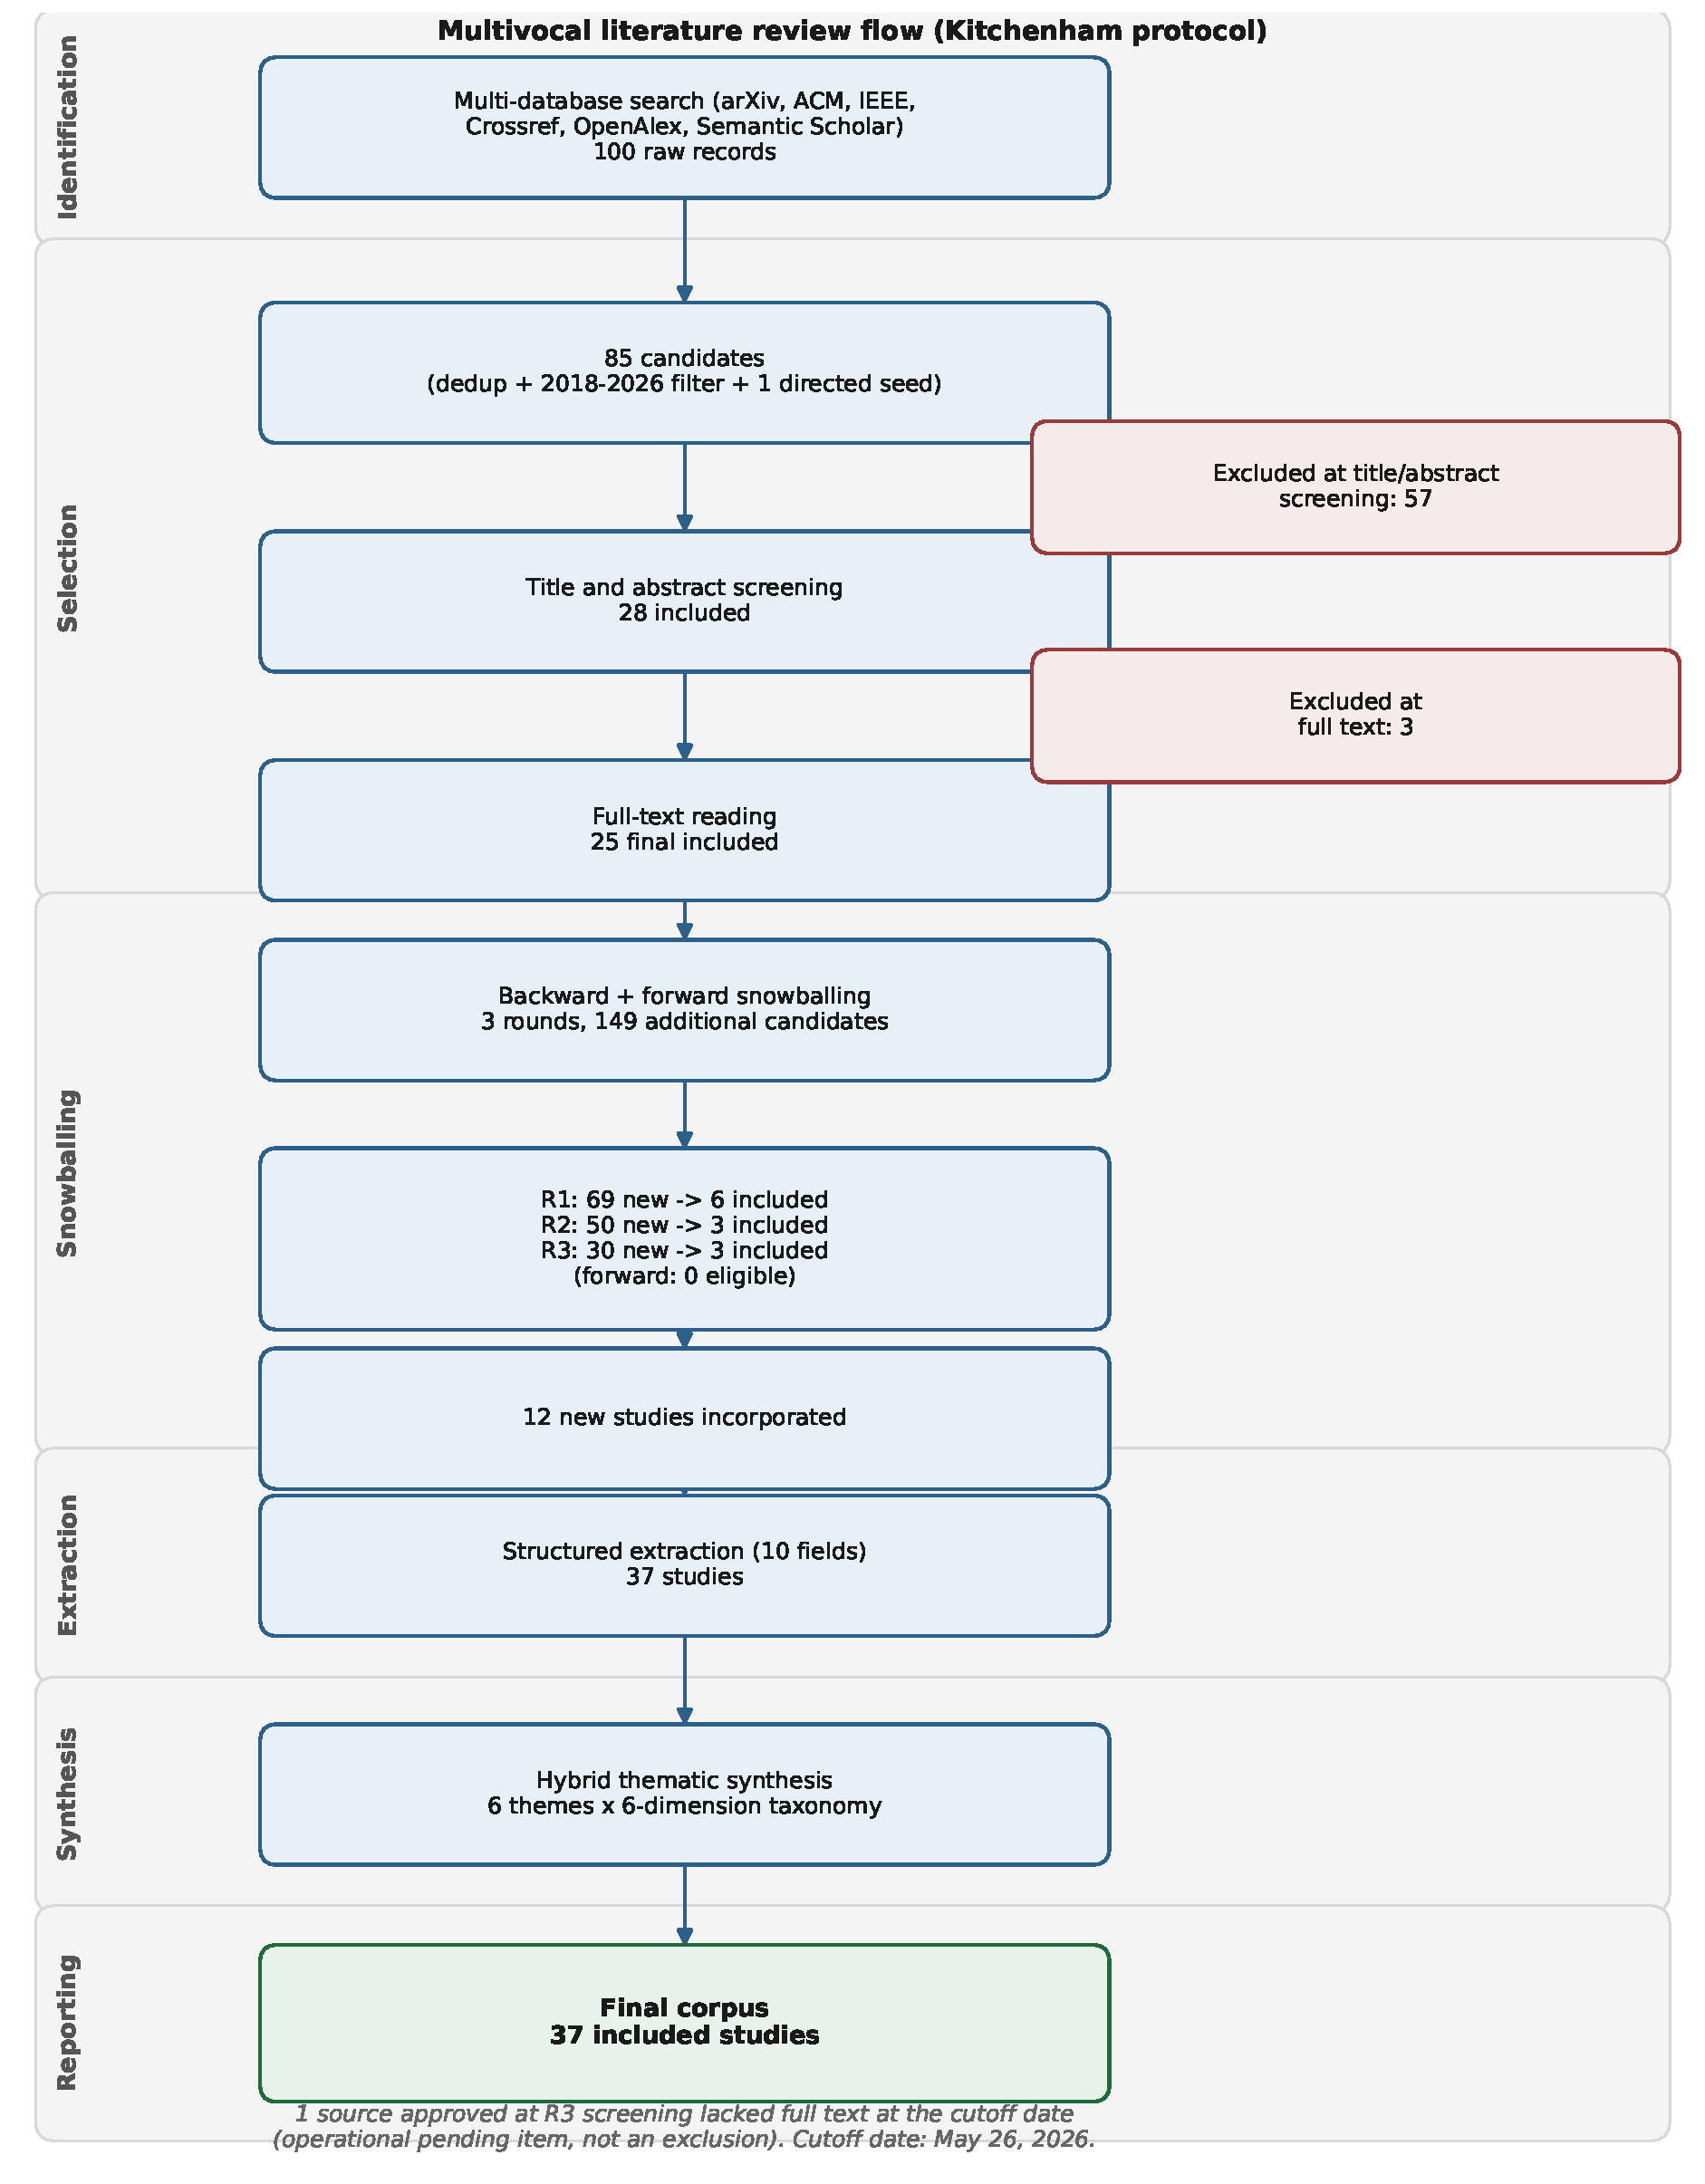
\includegraphics[width=0.92\textwidth]{methodology_en.pdf}
\caption{Systematic literature review flow, from the Kitchenham protocol to reporting, with the real counts at each step.}
\label{fig:metodologia}
\end{figure}

The review is guided by the five research questions presented in the Introduction (RQ1 through RQ5). RQ5, about the gaps that remain for comparing, evaluating, and governing these frameworks in real projects, is a synthesis-level question answered transversally in the Research Agenda, which is why the extraction matrix records only RQ1 through RQ4 per study.

The search was automated across arXiv, the ACM Digital Library, IEEE Xplore, Crossref, OpenAlex, and Semantic Scholar, with Scopus and Web of Science reached through open metadata via OpenAlex and Google Scholar used for citation checking. The descriptors were organized into four conceptual blocks (AI-assisted development, agentic software engineering, specification as artifact, and organization by workflows), with Boolean strings adapted to each database and documented in the protocol. In line with standard systematic-review practice, the candidate set also received one directed seed: a study within the initial scope, known to the authors and bearing a citable paper, that the automatic retrieval had missed.

The eligibility criteria were fixed in the protocol and are summarized in Table~\ref{tab:criterios}. The decision rule is aggregate: a source that fails criterion I1 is excluded; among sources that satisfy I1, only those that satisfy at least two of I2, I3, and I4 are included. Exclusion reasons were recorded operationally for each discarded source, allowing an auditable account of the discards in each pass.

\begin{table}[h!]
\centering
\caption{Inclusion and exclusion criteria applied in study selection.}
\label{tab:criterios}
\small
\begin{tabularx}{\textwidth}{@{}p{0.46\textwidth}Y@{}}
\toprule
\textbf{Inclusion criteria} & \textbf{Exclusion criteria} \\
\midrule
I1: describes a framework, method, toolkit, platform, IDE, CLI, or kit that organizes AI development across more than one step. & E1: addresses only language models, APIs, or code benchmarks, with no process layer. \\
I2: describes production or consumption of persistent artifacts (specs, plans, PRDs, tasks, logs, evidence). & E2: describes a generic code assistant, with no persistent artifacts, roles, commands, or validation of its own. \\
I3: defines roles, agents, personas, skills, workflows, or coordination commands. & E3: discusses LLMs for a single isolated task, with no framework or process proposal. \\
I4: describes integration with code execution, tests, terminal, IDE, browser, or repositories. & E4: is purely promotional, with no criteria, architecture, or traceable evidence. \\
I5: is an academic paper or archived preprint that is technically verifiable and citable. & E5: is a duplicate of a more complete or more recent source. \\
I6: available in English or Portuguese. & E6: has no citable paper, or is inaccessible for verification. \\
I7: published or updated between 2018 and 2026. & E7: is only an abstract, slide, brief announcement, or opinion without technical detail. \\
I8: allows at least four fields of the extraction schema to be extracted. & E8: mentions the frameworks only tangentially, with no substantive analysis. \\
\bottomrule
\end{tabularx}
\end{table}

The multi-database search returned 100 raw records, reduced to 85 candidates after deduplication by DOI and title, the 2018 to 2026 temporal filter, and the one directed seed described above. These 85 candidates went through a first title-and-abstract screening, which advanced 28 studies to full-text reading and excluded 57. In the second pass, the 28 full texts were read in full under the same criteria, yielding 25 included studies and 3 excluded. The counts and exclusion reasons for both passes were recorded in an append-only log for auditing.

From the 25 included studies, we applied backward and forward snowballing following Wohlin's guidelines \cite{wohlin2014snowballing}, with one depth level and a limit of three rounds, each seeded by the previous round's inclusions. The three rounds generated 69, 50, and 30 new candidates, respectively; of these, 9, 5, and 4 advanced to full text and 6, 3, and 3 were included, and the forward search returned no eligible citations in any round. In total, 149 additional candidates were examined and 12 new studies incorporated, consolidating the final corpus at 37 included studies. One source approved at the third-round screening lacked full text at the cutoff date and was kept as an operational pending item, not an exclusion.

Ten structured fields were extracted from each included study: name, nature, origin, artifacts, roles, execution, validation, portability, evidence, and risks. Consolidating the extraction into a matrix allowed the studies to be compared uniformly. The synthesis followed a hybrid thematic approach: inductive themes were identified from the extraction records and then confronted with the six-dimension taxonomy proposed in the review (specification, context, roles, execution, validation, and portability), reporting the overlap, the thinly covered dimensions, and the themes that emerge outside the taxonomy.

Finally, note that a formal quality assessment by checklist was not applied in this round: the strength of the evidence is classified by source category, distinguishing peer-reviewed study, conceptual paper, and archived preprint. Because the field moves quickly, observations about a study's reported versions, integrations, or tooling should be read as a snapshot of the corpus consulted at the cutoff date. The remaining limitations that bound the reading of the results are consolidated in the Review Limitations section.

\section{Related Work}

The literature that precedes this review falls into two strands, and the positioning of this study follows from the gap between them.

\noindent\textbf{Reviews of agents and AI software engineering.} The first strand gathers reviews and visions that map the use of language models and agents in software engineering. Hou et al. carry out a broad systematic review of language-model use across software engineering tasks, organized by lifecycle stage and by technique \cite{hou2024llmse}; He, Treude, and Lo review the internal architecture and cooperation of language-model multi-agent systems, drawing a roadmap toward consolidating them \cite{JundaHe2025}; and Hassan et al. propose a vision of AI-native software engineering, with a challenge roadmap for what they call Software Engineering 3.0 \cite{AhmedEHassan2024}. These contributions are valuable for understanding the anatomy of agents and the direction of the field. But they operate at a level of abstraction that classifies models, cognitive components, and techniques by task, or that projects future scenarios. None characterizes the operational frameworks that, today, organize development work on top of an agent at the level of process and repository.

\noindent\textbf{Process-oriented proposals.} The second strand is made of the frameworks that structure the process themselves. Spec-driven development articulates the specification as a living contract in the age of coding assistants \cite{DeepakBabuPiskala2026}; the distinction between vibe coding and agentic coding formalizes a spectrum of autonomy with practical implications \cite{RanjanSapkota2025}; and frameworks such as MetaGPT, ChatDev, and Reversa instantiate, each in its own way, the organization of the cycle around roles, artifacts, and validation \cite{SiruiHong2023,ChenQian2023,Macedo2026}. Each of these proposals, however, evaluates itself in isolation, with no common reference that would allow them to be compared.

\noindent\textbf{Positioning.} Between a review literature that describes agents abstractly and a proposal literature that evaluates each framework on its own, what is missing is a systematic review that takes the operational frameworks as its object, through a software engineering lens, and that confronts their structure with the available evidence through an explicit reference. That is the contribution of this article: a six-dimension taxonomy validated empirically against a corpus of 37 studies, a thematic synthesis that exposes the field's axes of tension, and a process-oriented research agenda. Unlike practitioner-facing product comparisons, the focus here is the body of literature and the structure that emerges from it, not the recommendation of a specific tool.

\section{Proposed Taxonomy}

To classify the corpus frameworks uniformly, we propose a taxonomy of six dimensions: specification, context, roles, execution, validation, and portability. These dimensions were chosen because they recur, under different names, across the studies analyzed, and they correspond to the structured fields extracted from each study. The taxonomy is presented here as a reference; its empirical validation against the corpus, including the strong dimensions and the weak ones, is reported in the Results section. Table~\ref{tab:taxonomia} summarizes each dimension through a guiding question and observable indicators.

\noindent\textbf{Specification.} Describes how the framework turns human intent into artifacts that guide the agent's work. At the weakest extreme, the specification is just a prompt; at the strongest, it is a versioned set of requirements, acceptance criteria, plans, tasks, architecture, and policies. Spec-driven development makes this dimension explicit by treating the specification as a versionable contract that drives generation \cite{DeepakBabuPiskala2026}, and AgileGen operationalizes it through executable acceptance criteria \cite{SaiZhang2025}. Reversa shifts the origin of the specification: instead of starting from a new product, it recovers operational specifications from existing systems \cite{Macedo2026}.

\noindent\textbf{Context.} The mechanism by which the framework decides what the agent should know before acting, which includes documents, code, history, architectural decisions, local rules, and collected evidence. Context engineering is treated as a discipline of its own for agents operating over real repositories \cite{SeyedmoeinMohsenimofidi2025}, and AutoCodeRover shows that structural retrieval of context from the code improves the quality of the patches generated \cite{YuntongZhang2024}. In Reversa, context is extracted from the legacy code and labeled by confidence \cite{Macedo2026}.

\noindent\textbf{Roles.} Define specialization, authority, and behavioral expectations. Multi-agent frameworks distribute tasks across personas such as product manager, architect, developer, tester, and reviewer, which reduces prompt ambiguity and sets output expectations. MetaGPT is the most explicit case, internalizing standard operating procedures and assigning specific artifacts to each role \cite{SiruiHong2023}, while ChatDev and CodePori show that role decomposition was already an active research line \cite{ChenQian2023,ZeeshanRasheed2024}.

\noindent\textbf{Execution.} Indicates whether the framework only produces guidance or also drives tools, edits code, runs tests, and interacts with interfaces. Modern agentic tools make execution a central dimension: the agent does not merely recommend, it modifies the environment. AutoDev and AutoCodeRover operate directly on the repository, editing code and running tests on real program-improvement tasks \cite{MicheleTufano2024,YuntongZhang2024}, and Prompt Sapper materializes execution as a production platform for AI chains \cite{YuCheng2023}.

\noindent\textbf{Validation.} Comprises the mechanisms for checking whether what was produced is correct, complete, and aligned with the context, which can include automated tests, human review, evidence artifacts, auditable traces, and readiness gates. Trace-based assurance articulates contracts, tests, and governance \cite{Paduraru2026}; verifiable collaboration among assistants makes every act in the flow auditable \cite{Merchant2025}; and Reversa makes confidence and gaps explicit in the recovered artifacts \cite{Macedo2026}. Validation is critical because agents can produce plausible results without real adherence to the system.

\noindent\textbf{Portability.} Describes whether the framework depends on a specific vendor, IDE, model, or format. In the corpus, this is the most fragile dimension: it appears almost always on the negative side, as a risk of lock-in and of dependence on a platform, and lock-in is named explicitly in only one study \cite{SeyedmoeinMohsenimofidi2025}. Almost no framework treats portability as a positive, deliberate design property, which is why it is best read as a predominantly diagnostic dimension, as detailed in the Results section.

\begin{table}[h!]
\centering
\caption{Dimensions of the proposed taxonomy.}
\label{tab:taxonomia}
\small
\begin{tabularx}{\textwidth}{p{2.8cm}Y Y}
\toprule
\textbf{Dimension} & \textbf{Guiding question} & \textbf{Observable indicators} \\
\midrule
Specification & How does intent become a work contract? & Specs, PRDs, plans, stories, tasks, acceptance criteria \\
Context & How does the agent know what is relevant? & Repository, docs, hooks, rules, memory, evidence, gaps \\
Roles & Who decides, who implements, who reviews? & Personas, agents, skills, responsibilities, authority \\
Execution & Does the framework act on the environment or only guide? & Code editing, commands, tests, browser, terminal, IDE \\
Validation & How are errors caught before they become deliverables? & Tests, checklists, gates, artifacts, human review, confidence \\
Portability & Does the process survive outside one tool? & Multiple integrations, open formats, lock-in, local install \\
\bottomrule
\end{tabularx}
\end{table}

\section{Results and Synthesis}

This section consolidates the findings of the 37 included studies. The synthesis follows a hybrid thematic approach: six themes were derived inductively from the structured fields of the extraction records (artifacts, roles, execution, validation, portability, risks, nature, and evidence) and then confronted with the six-dimension taxonomy proposed in the previous section, so as to test it against the evidence rather than assume it. The themes answer RQ1 through RQ4; RQ5, on gaps, is addressed in the Research Agenda. The strength of each study's evidence is weighted by a source-category quality assessment, described in the Method and summarized below (Table~\ref{tab:qualidade}).

\noindent\textbf{Quantitative overview.} Table~\ref{tab:quant} summarizes the composition of the corpus. The framework category dominates almost entirely (34 of the 37 studies), which empirically supports the thesis that the unit of work has shifted from the isolated prompt to the structured process. Empirical evaluation is claimed by 26 studies and 22 release a public repository, but ten are arXiv preprints not yet peer-reviewed, which calls for a qualified reading of the strength of the evidence (Figure~\ref{fig:evidence}). The temporal distribution shows steady acceleration of the field, from a single study in 2022 to eleven in 2026, with most of the corpus concentrated from 2024 onward (Figure~\ref{fig:year}). Venues are dispersed, with the ACM Transactions on Software Engineering and Methodology as a recurring outlet (five studies) followed by a long tail of conferences and journals with one or two studies each, consistent with an emerging field that still lacks a consolidated forum.

\begin{table}[h!]
\centering
\caption{Composition of the corpus of 37 included studies. Counts extracted from the extraction matrix.}
\label{tab:quant}
\small
\begin{tabularx}{\textwidth}{@{}p{0.50\textwidth}r Y@{}}
\toprule
\textbf{Aspect} & \textbf{N} & \textbf{Note} \\
\midrule
Total included studies & 37 & After two screening passes and three snowballing rounds \\
Nature: framework & 34 & Near-total predominance \\
Nature: architecture / platform / method & 1 / 1 / 1 & JulesWhite2023, YuCheng2023, JSauvola2024 \\
With empirical evaluation & 26 & Some degree of validation claimed \\
With public repository & 22 & Code traceability in more than half \\
arXiv preprint & 10 & Literature not yet peer-reviewed \\
Survey or review & 2 & AhmedEHassan2024, JundaHe2025 \\
Case study & 5 & Ulfsnes2024, ZeeshanRasheed2024, Baron2025, Khan2026, Macedo2026 \\
Distribution by year & \multicolumn{2}{l}{2022:1, 2023:4, 2024:10, 2025:11, 2026:11} \\
Academic or technical / industrial origin & 33 / 4 & Four studies from industry or professional practice \\
High extraction confidence & 35 & Medium in Dam2025 and JundaHe2025 \\
\bottomrule
\end{tabularx}
\end{table}

\begin{figure}[h!]
\centering
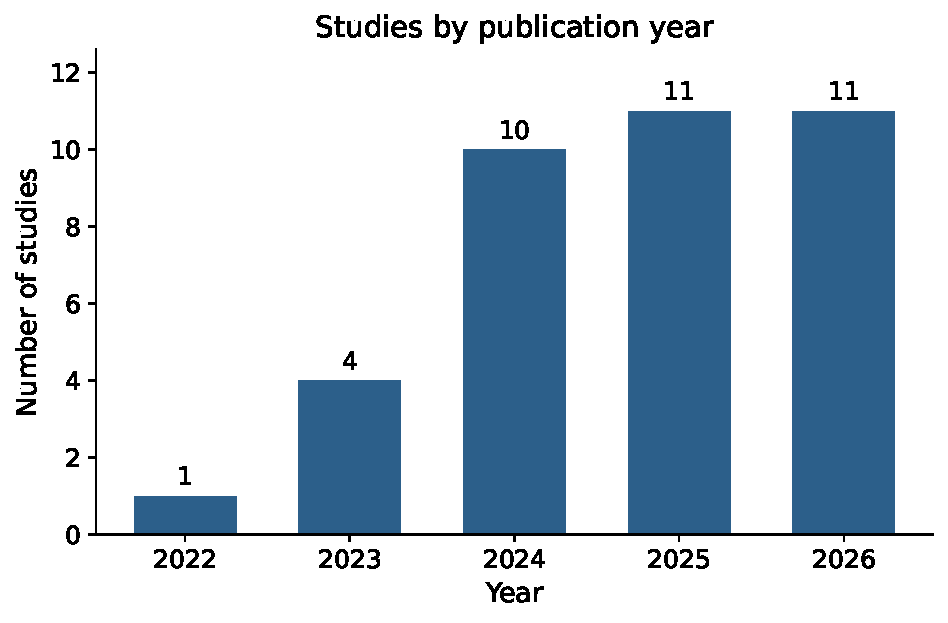
\includegraphics[width=0.70\textwidth]{studies_by_year_en.pdf}
\caption{Studies by publication year. The field accelerates from a single study in 2022 to a plateau of ten to eleven per year from 2024 onward.}
\label{fig:year}
\end{figure}

\begin{figure}[h!]
\centering
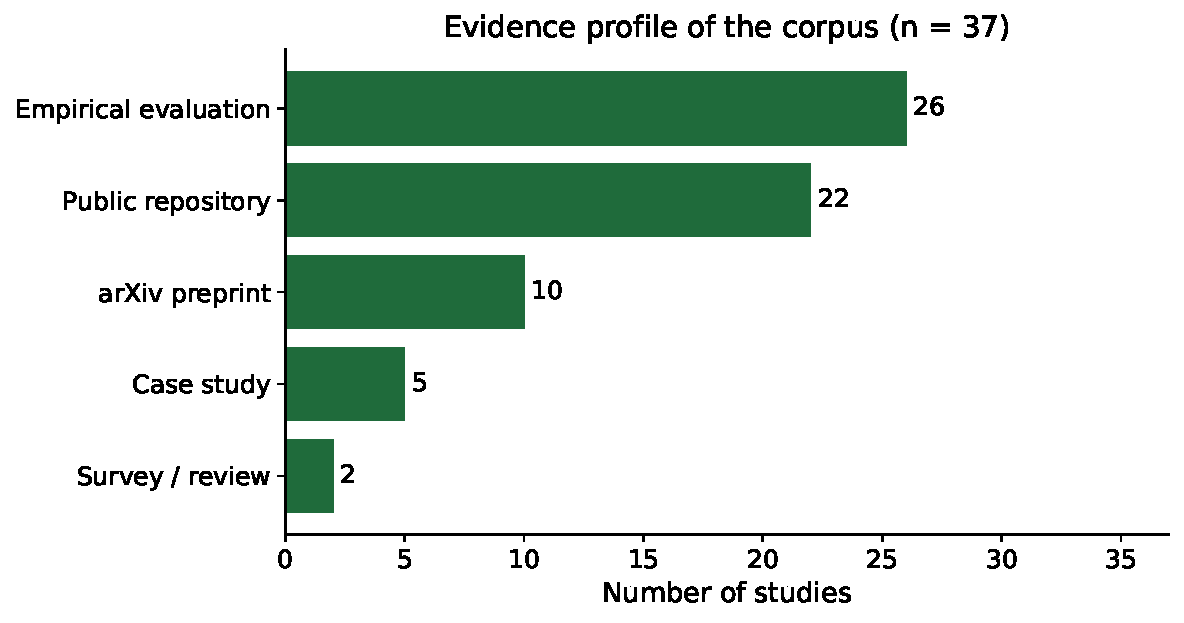
\includegraphics[width=0.80\textwidth]{evidence_profile_en.pdf}
\caption{Evidence profile of the corpus. Most studies claim empirical evaluation and release a public repository, but ten are arXiv preprints not yet peer-reviewed.}
\label{fig:evidence}
\end{figure}

\noindent\textbf{Quality assessment by source category.} Table~\ref{tab:qualidade} summarizes the quality assessment described in the Method, with the four-item checklist applied to the 37 studies. Eleven studies (30\%) fall in the high-quality band, seventeen (46\%) in the medium band, and nine (24\%) in the low band. Most of the corpus comes from peer-reviewed venues (25 studies, 68\%), against ten arXiv preprints (27\%) and two non-indexed technical records (5\%). At the item level, 26 studies (70\%) report empirical evaluation and 22 (59\%) release a public repository, but only five (14\%) bring applied validation in a case study or real project, which bounds how far the current evidence supports production use. The low band concentrates preprints and technical records without recorded empirical evaluation; their findings are read cautiously in the synthesis and no theme rests exclusively on them. The assessment is conservative by construction, since it derives from the signals recorded in the extraction rather than from a full-text reappraisal of each study.

\begin{table}[h!]
\centering
\caption{Source-category quality assessment of the 37 studies. Items derived from observable signals in the extraction matrix; QA is the sum of QA1 to QA4 (0 to 4).}
\label{tab:qualidade}
\small
\begin{tabularx}{\textwidth}{@{}p{0.46\textwidth}r Y@{}}
\toprule
\textbf{Category} & \textbf{N} & \textbf{\%} \\
\midrule
High quality (QA $\geq$ 3) & 11 & 30\% \\
Medium quality (QA = 2) & 17 & 46\% \\
Low quality (QA $\leq$ 1) & 9 & 24\% \\
\midrule
Peer-reviewed venue (QA1) & 25 & 68\% \\
arXiv preprint & 10 & 27\% \\
Non-indexed technical record & 2 & 5\% \\
\midrule
Reported empirical evaluation (QA2) & 26 & 70\% \\
Applied validation in a case study (QA3) & 5 & 14\% \\
Public artifact for reproducibility (QA4) & 22 & 59\% \\
\bottomrule
\end{tabularx}
\end{table}

\noindent\textbf{Six inductive themes.} The analysis surfaced six themes that, together, cover the 37 studies (100\% coverage, above the 80\% target). Each study may belong to more than one theme; the order reflects decreasing frequency.

\noindent\textbf{T1: multi-agent orchestration and role division.} This is the most populous theme and the dominant architectural axis of the corpus, answering RQ1 directly. The central convergence is that structuring the work by distinct roles, not the choice of language model, is what differentiates the frameworks. ChatDev encodes a chat chain with design, coding, testing, and review phases, plus a communicative dehallucination mechanism \cite{ChenQian2023}. MetaGPT internalizes standard operating procedures from software engineering, assigning specific artifacts to each role: the product manager generates requirements, the architect generates the design and interfaces, the developer implements \cite{SiruiHong2023}. CodePori scales that arrangement to agents for management, architecture, structure, development, verification, and finalization \cite{ZeeshanRasheed2024}, and AutoDev and AutoCodeRover bring agent coordination to real program-improvement tasks \cite{MicheleTufano2024,YuntongZhang2024}. He et al.'s reviews and Hassan et al.'s Software Engineering 3.0 vision confirm that the literature already organizes these systems by lifecycle stage \cite{JundaHe2025,AhmedEHassan2024}. Consensus, however, is partial: there is clear tension over the degree of autonomy. Sapkota et al. explicitly contrast vibe coding and agentic coding \cite{RanjanSapkota2025}, and while CodePori and MetaGPT lean toward end-to-end autonomous development, other designs preserve human decision points. Reliability and coordination cost appear as recurring risks in this theme \cite{Dam2025,Alsegier2026,Merchant2025,Paduraru2026,SKaruppuchamy2026,Paiva2026,Akbar2025,LiyiCai2025,Anon2026,BESLEAGA2026}.

\noindent\textbf{T2: specification and contract as the central artifact.} This theme answers RQ1 and RQ2 and gives substance to the thesis that the specification becomes the unit of coordination. Spec-driven development formalizes the move from code to contract, treating the specification as a versionable artifact \cite{DeepakBabuPiskala2026}. AgileGen uses acceptance criteria as an executable contract and keeps memory and iteration until validation \cite{SaiZhang2025}, and MetaGPT already made structured requirements the source of truth across roles \cite{SiruiHong2023}. There is, however, a productive contradiction in the direction of the flow: most assume spec-first, where the specification precedes and generates the code, whereas Reversa inverts the flow, recovering operational specifications from legacy code to feed the agents \cite{Macedo2026}. This opposition between specifying first and recovering the specification from legacy is a relevant axis of differentiation. Risk-aware requirements engineering ties the specification to governance \cite{Watfa2026}, and the misalignment between specification and code is discussed as a risk across several studies \cite{DeepakBabuPiskala2026,Paduraru2026,Watfa2026,YuCheng2023,Gupta2022,MitulModi2024,Khan2026,Gadamsetty2025}.

\noindent\textbf{T3: context engineering and repository knowledge retrieval.} This theme answers RQ2 with a focus on the context dimension. Context engineering is treated as a discipline of its own for agents in open-source software \cite{SeyedmoeinMohsenimofidi2025}. AutoCodeRover shows that structural retrieval of context from the code, and not just textual search by embeddings, improves patch generation \cite{YuntongZhang2024}, while the synchronization of multimodal artifacts seeks to keep coherence across heterogeneous artifacts over the cycle \cite{Paiva2026}. Self-evolving software pushes the theme to its extreme \cite{LiyiCai2025}, but it sits in tension with the emphasis on traceability and contract in T2 and T4: the more the software modifies itself autonomously, the harder it is to anchor each change in an auditable specification \cite{Macedo2026,AhmedEHassan2024,Chechik2026}. The risk tied to context is the most frequent in the whole corpus, which suggests that the context window and context fidelity are the transversal practical bottleneck of the field.

\noindent\textbf{T4: validation, traceability, assurance, and governance.} This theme answers RQ2, in the validation dimension, and RQ4, in the risks of governance and traceability. Almost the entire corpus declares some validation mechanism, but here we group the studies for which validation is the central point rather than an appendix. Trace-based assurance articulates contracts, tests, and governance \cite{Paduraru2026}; verifiable collaboration among agentic assistants records the acts of the flow in an auditable way \cite{Merchant2025}; and product-line engineering is imported to govern the variability of agency \cite{Alsegier2026}. Traceability and trace auditing appear as a recurring requirement for trusting agents on real projects \cite{Paduraru2026,Merchant2025,Macedo2026,SKaruppuchamy2026,Watfa2026,Chechik2026,Anon2026}. There is, however, a cost contradiction: on one side, heavy governance ceremony \cite{Merchant2025,Paduraru2026}; on the other, lightweight agility aimed at startups and lean flows \cite{Khan2026,RanjanSapkota2025,JulesWhite2023}. Coordination cost is named as a risk in much of this group \cite{MitulModi2024,Ulfsnes2024,Akbar2025,Baron2025,KRRaghi2024,Gupta2022,KumarAle2024}, which materializes the tension between governance and productivity.

\noindent\textbf{T5: human-AI collaboration, adoption, and trust (emergent).} These studies focus not on the technical architecture but on integrating AI into human work: collaboration flows, organizational adoption factors, and trust building. A human-AI collaboration and adaptation framework models workflow factors and organizational strategies \cite{DanielRusso2024}; field evidence describes how real teams reorganize collaboration and flow \cite{Ulfsnes2024,Akbar2025}; and trust is treated as a precondition for adoption \cite{Baron2025}, with future scenarios of AI-assisted operation also documented \cite{JSauvola2024}. The notable finding is that this theme does not fit cleanly into any of the six taxonomy dimensions, all of which are technical and architectural: the human, organizational, and trust dimension cuts across the corpus but has no home in the current taxonomy. Six studies (16\% of the corpus) have this as their primary focus, enough to recommend extending the taxonomy.

\noindent\textbf{T6: security, robustness, and red-teaming (emergent).} These studies focus on the security of the code and of agentic behavior. ASTRA proposes autonomous spatial-temporal red-teaming for AI software assistants, treating security as an active activity rather than an assumed property \cite{XiangzheXu2025}; risk-aware requirements engineering and the discussion of the security implications of agentic coding reinforce the theme \cite{Watfa2026,RanjanSapkota2025,Merchant2025,BESLEAGA2026}, and ChatDev's communicative dehallucination touches the point from the reliability side \cite{ChenQian2023}. Security is among the most frequently cited risks, named in 24 of the 37 studies, behind context, reliability, and coordination cost (Figure~\ref{fig:risk}). Like T5, this theme connects only partially to the six dimensions: security appears almost always as a risk to mitigate, rarely as a positive design dimension embedded in the architecture. ASTRA is the exception that makes security the central object, which suggests treating it as a transversal evaluation criterion rather than as one of the dimensions that classify frameworks.

\begin{figure}[h!]
\centering
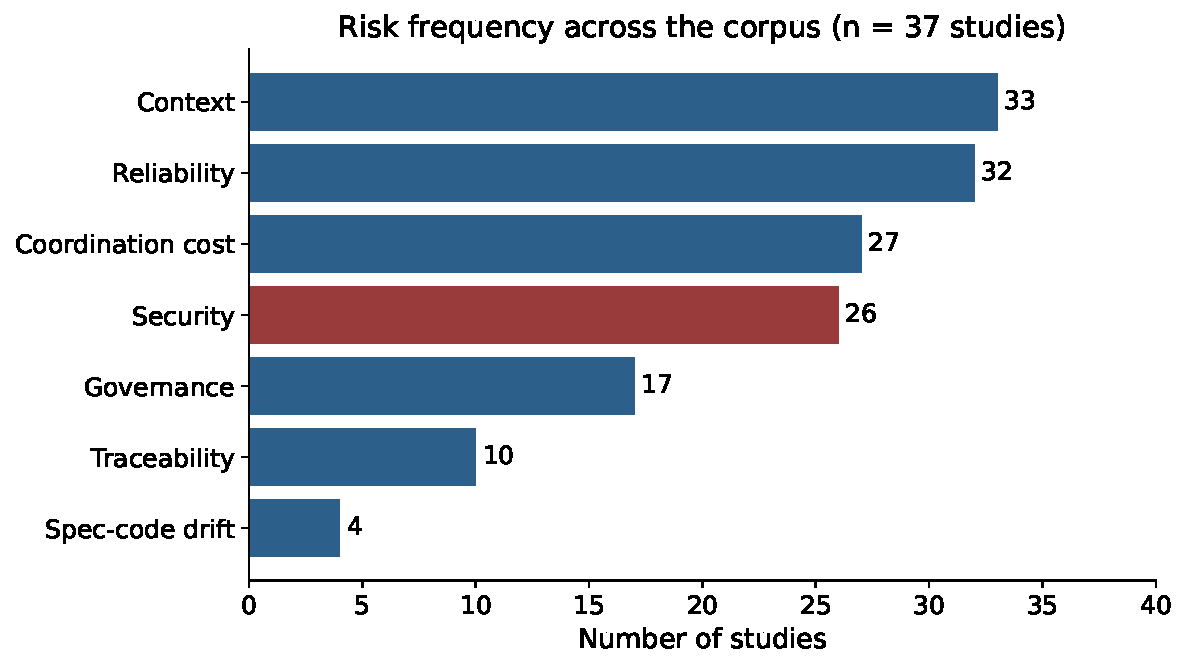
\includegraphics[width=0.80\textwidth]{risk_frequency_en.pdf}
\caption{Frequency of reported risks across the corpus. Context, reliability, and coordination cost lead; security, though prominent, ranks below them, and explicit lock-in tagging is rare.}
\label{fig:risk}
\end{figure}

\noindent\textbf{Confronting the taxonomy with the evidence.} Table~\ref{tab:tema-dim} crosses each inductive theme with the six taxonomy dimensions, indicating the strength of the relation, which is coded by the author from the extraction records. The reading is direct. Five of the six dimensions receive strong support from at least one theme: roles and execution anchor in T1; specification and validation, in T2 and T4; context, in T3. In that part, the taxonomy holds up against the evidence. Figure~\ref{fig:heatmap} renders the same mapping as a heatmap. The exception is portability, which receives no strong relation from any theme and is absent in two. In the data, portability appears almost always on the negative side, as a risk of lock-in and of dependence on an IDE, a commercial model, or a platform. The portability field of the records notes dependence on an IDE or environment in nearly all 37 studies, and lock-in is named explicitly as a risk in only one of them \cite{SeyedmoeinMohsenimofidi2025}. Portability is therefore the weakest dimension of the taxonomy when confronted with the evidence, and should be read as a predominantly diagnostic dimension, not as a positive differentiator between frameworks. Themes T5 and T6, in turn, have no clear home in the six dimensions: the human-organizational axis and the security axis emerge from the data as concrete recommendations for extension, and the rule of the hybrid mode was respected by not forcing them into the existing dimensions.

\begin{table}[h!]
\centering
\caption{Hybrid mapping: inductive themes against the six taxonomy dimensions. Legend: strong (the dimension is the theme's axis), medium (relevant presence), weak (marginal touch), absent (no significant relation).}
\label{tab:tema-dim}
\small
\begin{tabularx}{\textwidth}{@{}p{3.5cm}YYYYYY@{}}
\toprule
\textbf{Theme} & \textbf{Spec.} & \textbf{Context} & \textbf{Roles} & \textbf{Exec.} & \textbf{Valid.} & \textbf{Portab.} \\
\midrule
T1 Multi-agent orchestration & medium & medium & strong & strong & medium & weak \\
T2 Specification and contract & strong & medium & weak & medium & strong & weak \\
T3 Context engineering & weak & strong & weak & medium & weak & weak \\
T4 Validation and governance & medium & weak & weak & medium & strong & weak \\
T5 Human-AI collaboration & weak & weak & weak & weak & weak & absent \\
T6 Security and red-teaming & weak & weak & weak & medium & medium & absent \\
\bottomrule
\end{tabularx}
\end{table}

\begin{figure}[h!]
\centering
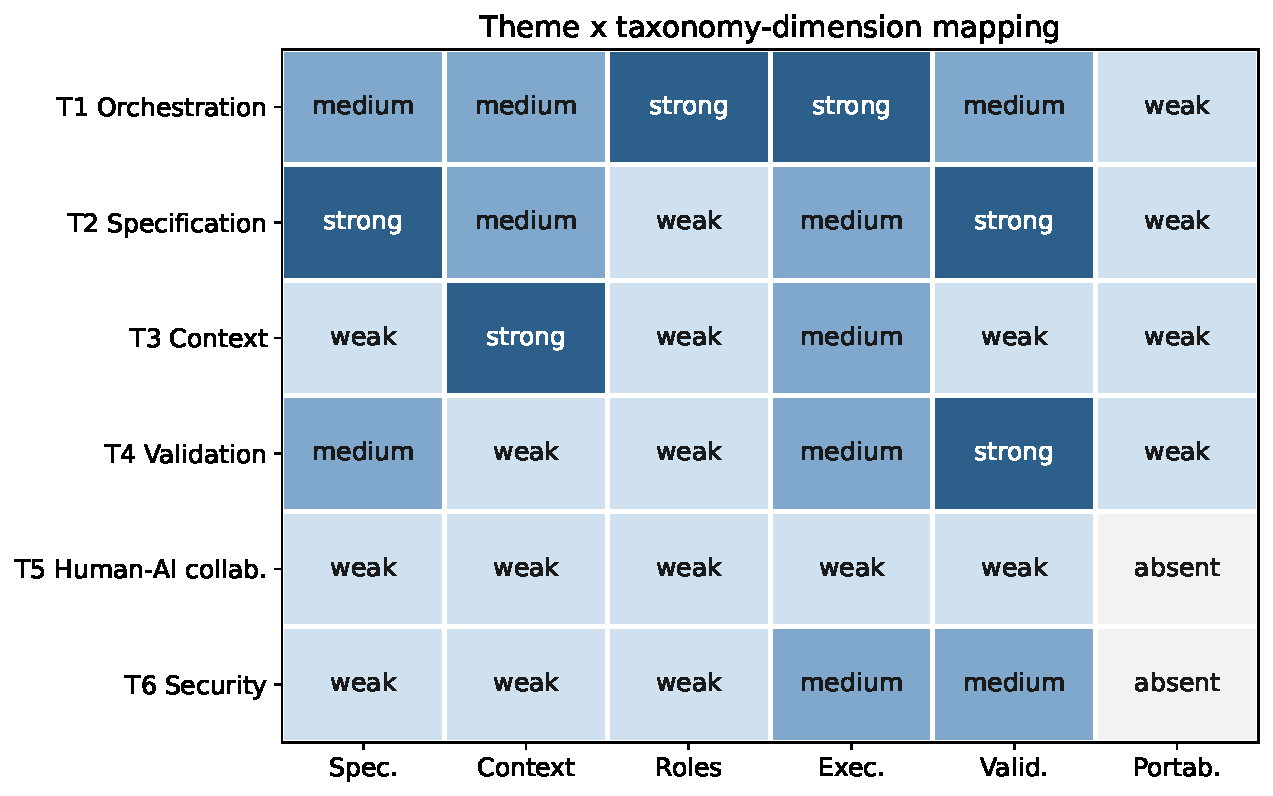
\includegraphics[width=0.92\textwidth]{theme_dimension_en.pdf}
\caption{Hybrid mapping of the six inductive themes against the six taxonomy dimensions. Five dimensions are anchored by at least one theme; portability stays weak throughout, and themes T5 and T6 fall partly outside the taxonomy.}
\label{fig:heatmap}
\end{figure}

\noindent\textbf{Coverage of the research questions.} Table~\ref{tab:tema-rq} crosses the themes with the research questions. RQ1 and RQ2 are answered by most themes; RQ3 and RQ4 cut across the whole corpus, and RQ5 is a meta-question answered transversally in the Research Agenda rather than by study-by-study tagging, which is why the individual records mark only RQ1 through RQ4.

\begin{table}[h!]
\centering
\caption{Inductive themes against the research questions.}
\label{tab:tema-rq}
\small
\begin{tabularx}{\textwidth}{@{}p{3.5cm}YYYYY@{}}
\toprule
\textbf{Theme} & \textbf{RQ1} & \textbf{RQ2} & \textbf{RQ3} & \textbf{RQ4} & \textbf{RQ5} \\
\midrule
T1 Multi-agent orchestration & yes & yes & yes & yes & via synthesis \\
T2 Specification and contract & yes & yes & partial & yes & via synthesis \\
T3 Context engineering & yes & yes & partial & yes & via synthesis \\
T4 Validation and governance & partial & yes & yes & yes & via synthesis \\
T5 Human-AI collaboration & partial & yes & yes & yes & via synthesis \\
T6 Security and red-teaming & no & partial & yes & yes & via synthesis \\
\bottomrule
\end{tabularx}
\end{table}

\section{Discussion}

The synthesis of the six themes supports four transversal readings that cut across the research questions and organize what the corpus, taken as a whole, tells us about the state of the field.

\noindent\textbf{The unit of work has shifted from prompt to process.} The central thesis of this study holds empirically. In 34 of the 37 studies the contribution is described as a framework, and the fields for persistent artifacts, roles, and validation are present in the vast majority of records. The language model is rarely the declared differentiator; what sets the proposals apart is the process structure that organizes specs, roles, execution, and validation around the agent's work. The three studies that are not frameworks reinforce the contrast: an architecture of prompt patterns, an AI-chain platform, and a method of future scenarios. These are exactly the cases where the unit is still the isolated technique and not the process \cite{JulesWhite2023,YuCheng2023,JSauvola2024}.

\noindent\textbf{The six-dimension taxonomy is partly validated and partly challenged.} Five dimensions (specification, context, roles, execution, and validation) have strong empirical anchoring in at least one theme. The sixth, portability, is weak and almost always diagnostic: it shows up as a risk of lock-in and platform dependence, not as a deliberate design property. Two relevant axes also emerge outside the six dimensions, the human-organizational one in T5 and the security one in T6. The analytical recommendation that follows from the hybrid mode is concrete: consider extending the taxonomy with a dimension of human-AI collaboration and governance, and treat security as a transversal evaluation criterion or a subdimension of validation. That is what confronting the themes with the taxonomy adds, compared to assuming the dimensions a priori.

\noindent\textbf{Three recurring axes of tension.} The corpus shows partial consensus, not convergence, along three axes. The first is autonomy versus human control: CodePori, MetaGPT, and ChatDev lean toward an end-to-end autonomous flow, while frameworks centered on adoption and trust build human decision in as a design element, and the distinction between vibe coding and agentic coding theorizes the contrast \cite{ZeeshanRasheed2024,SiruiHong2023,ChenQian2023,SaiZhang2025,DanielRusso2024,Baron2025,RanjanSapkota2025}. The second is heavy governance versus lightweight agility: verification ceremonies and formal contracts stand against lean flows for startups and prompt patterns, and coordination cost is the recurring price of governance \cite{Merchant2025,Paduraru2026,Khan2026,JulesWhite2023}. The third is the direction of the specification flow: specifying first, in spec-driven development, MetaGPT, and AgileGen, versus recovering the specification from legacy, in Reversa \cite{DeepakBabuPiskala2026,SiruiHong2023,SaiZhang2025,Macedo2026}. The two extremes anchor in the same specification dimension but in opposite directions, which is material for any future comparative matrix.

\noindent\textbf{Traceability and context are the most cited transversal requirements.} The risk tied to context appears in nearly every study, and traceability is a recurring demand in the specification and governance themes. Together, they indicate that the field's practical bottlenecks are not in code generation itself, but in keeping the agent anchored in the real project and auditable over time. This finding realigns the usual reading of the problem: the open challenge is less about producing plausible code and more about sustaining fidelity to the system and to the recorded intent.

\noindent\textbf{The evidence is uneven.} Although 26 of the 37 studies declare empirical evaluation and 22 have a public repository, ten are arXiv preprints not yet peer-reviewed, and most evaluations occur on benchmarks or one-off case studies, not on longitudinal industrial projects. The strength of the evidence varies widely by source category, exactly as the protocol anticipated by classifying evidence by category instead of applying quality-based exclusion. This heterogeneity calls for caution: the findings of this study describe the structure and tensions of the field with confidence, but claims about relative performance between frameworks remain underdetermined by the available evidence.

\section{Research Agenda}

RQ5 asks which gaps remain for comparing, evaluating, and governing these frameworks in real projects. Unlike the other questions, it is answered at the level of the whole corpus rather than study by study. Six gaps emerge from the synthesis, each with a concrete research direction.

\noindent\textbf{Absence of process-oriented benchmarks.} The corpus evaluation concentrates on the final result, that is, the generated code and the issue-resolution rate, not on process quality: adherence of the implementation to the specification, drift rate, coordination cost between agents, and quality of intermediate artifacts. No study proposes a standardized process benchmark. The direction indicated is to define metrics and datasets that evaluate the pipeline, not just the solution.

\noindent\textbf{Lack of direct empirical comparison between frameworks.} Each study evaluates its own framework in isolation. There is no controlled comparative study that pits, say, ChatDev, MetaGPT, and AgileGen against the same task with the same metrics \cite{ChenQian2023,SiruiHong2023,SaiZhang2025}. This blocks conclusions about which process structure works best and under which conditions. The direction indicated is head-to-head comparative experiments with common protocols.

\noindent\textbf{Portability and lock-in, little studied as an object.} Dependence on an IDE, a platform, and a commercial model is nearly universal in the records, but only one study names lock-in explicitly, and none measures portability systematically \cite{SeyedmoeinMohsenimofidi2025}. The direction indicated is instruments to measure vendor coupling and the cost of migrating between agentic platforms.

\noindent\textbf{Governance and traceability lack validation at real scale.} The proposals for traces, contracts, and auditing are promising but validated on case studies or prototypes, not on organizations over time, and there is no cost-benefit analysis of the coordination cost imposed by governance \cite{Paduraru2026,Merchant2025,Watfa2026,Macedo2026}. The direction indicated is the longitudinal evaluation of governance regimes in real teams.

\noindent\textbf{The human and adoption dimension is underrepresented in the technical taxonomy.} The emergent collaboration theme shows that trust and organizational adoption are decisive, but the six-dimension taxonomy does not account for them \cite{DanielRusso2024,Ulfsnes2024,Baron2025,Akbar2025}. The direction indicated is to integrate a sociotechnical layer into the classification of frameworks and to study adoption factors in the field.

\noindent\textbf{Security treated reactively.} With the exception of ASTRA, security appears as a risk to mitigate, not as an evaluated design property \cite{XiangzheXu2025}. There is no systematic evaluation of the attack surface of agentic frameworks, especially of community extensions, skills, and plugins. The direction indicated is a security evaluation framework specific to agentic development pipelines.

\section{Review Limitations}

Five limitations bound the reading of the results and qualify the reach of the conclusions.

\noindent\textbf{Extraction granularity.} The thematic synthesis derives from the structured fields of the records (artifacts, roles, execution, validation, portability, risks, nature, and evidence) and from a consolidated narrative finding per study, produced in a second extraction pass. Twelve studies have a finding drawn from a substantive inclusion justification, and the other twenty-five receive a finding consolidated from the structured fields, transparently flagged as such. Where the first-pass justification is generic, the reading still rests in part on the known public identity of well-documented frameworks, such as ChatDev, MetaGPT, AutoCodeRover, Reversa, and AgileGen. A full-text, field-by-field extraction for the remaining twenty-five studies would deepen the synthesis further.

\noindent\textbf{Quality assessment by category, not by full text.} We applied a four-item source-category quality assessment (Table~\ref{tab:qualidade}) that weights the strength of the evidence and flags the lower-confidence studies, but it does not replace a formal risk-of-bias instrument applied to the full text of each study. The ten arXiv preprints not yet peer-reviewed and the two studies with medium extraction confidence enter the synthesis with a cautious reading, and no theme rests exclusively on them; even so, a full-text reappraisal with a validated instrument would refine the weighting.

\noindent\textbf{Language and database scope, and publication bias.} The protocol restricts the review to English and Portuguese, in the 2018 to 2026 window. The direct arXiv search failed in part due to access instability, with preprint coverage recovered via Semantic Scholar and the arXiv DOI, which may have left out very recent preprints not indexed by those routes. A publication bias toward frameworks with positive results is likely and measurable in the corpus itself: 26 of the 37 studies (70\%) claim empirical evaluation, almost always favorable to the proposed framework, while studies of failure, abandonment, or non-adoption are practically absent; only the adoption axis of theme T5, with six studies, problematizes organizational integration. Widening the search to additional databases and lifting the language restriction is future work that could balance this asymmetry.

\noindent\textbf{Operational pending item outside the corpus.} One source approved at screening lacked full text obtained at the cutoff date and was kept as an operational pending item, outside the extraction and this synthesis. The corpus effectively synthesized is 37 studies; incorporating that source later would adjust marginal counts without changing the thematic structure.

\noindent\textbf{Partial snowballing saturation.} Snowballing was stopped at the protocol limit of three rounds. The saturation curve (Figure~\ref{fig:saturacao}) shows decreasing inclusions, from 25 in the initial search to 6, 3, and 3 across the three rounds: a clear but nonzero deceleration. The last rounds still added studies, which indicates partial rather than full saturation; additional rounds could surface relevant studies, especially outside the communities of origin of the seeds.

\section{Conclusion}

This review systematized 41 studies on AI-assisted software development frameworks that shift the unit of work from the isolated prompt to a structured process, with persistent artifacts, agentic roles, integrated execution, and validation. The thesis that this shift has already happened rests on the evidence: the contribution is described as a framework in 37 of the 41 studies, and the declared differentiator is the process structure, not the underlying language model. On that corpus, we proposed and tested a six-dimension taxonomy. Five dimensions (specification, context, roles, execution, and validation) receive strong empirical support; portability is weak and predominantly diagnostic, and two relevant axes, the human-organizational and the security one, emerge outside the taxonomy and recommend extending it.

The field is young, has accelerated since 2024, and still lacks a consolidated publication forum, which is reflected in the dispersion of venues and the sizable presence of preprints. The evidence is uneven, and three axes of tension (autonomy versus human control, heavy governance versus lightweight agility, and specifying first versus recovering the specification from legacy) structure the debate without resolving it. The most cited practical bottlenecks are not in code generation but in keeping the agent anchored in the real project and auditable: context and traceability are the dominant transversal requirements.

The consequence for future research is direct. The field's next step is empirical and process-oriented: benchmarks that evaluate the pipeline and not only the solution, direct comparisons between frameworks, portability instruments, longitudinal evaluation of governance, a sociotechnical layer in the classification, and systematic security evaluation. This review offers the validated taxonomy and the agenda that organize that effort.

\appendix
\section{Reporting Compliance Checklist}
\label{ap:checklist}

Table~\ref{tab:checklist} lists the reporting items recommended for systematic reviews under the Kitchenham and Charters guidelines \cite{kitchenham2009slr}, indicating, for each item, where it is reported in this article. The goal is to make reporting compliance auditable and to ease replication. The protocol artifacts, the screening logs, the extraction matrix, the quality assessment, and the figure and reliability scripts are available in the study repository.

\begin{table}[h!]
\centering
\caption{Kitchenham reporting checklist and where each item is met in this article.}
\label{tab:checklist}
\small
\begin{tabularx}{\textwidth}{@{}p{0.50\textwidth}Y@{}}
\toprule
\textbf{Reporting item} & \textbf{Where it is met} \\
\midrule
Review context and rationale & Introduction \\
Research questions (RQ1 to RQ5) & Introduction; Review Method \\
Protocol fixed before execution & Review Method; \texttt{protocol.md} \\
Sources consulted and search strings & Review Method; \texttt{descriptors.md} \\
Inclusion and exclusion criteria & Review Method (criteria table) \\
Two-pass selection and counts & Review Method; logs in \texttt{screening/} \\
Snowballing and saturation analysis & Review Method (saturation figure) \\
Inter-rater reliability (IRR) & Review Method; \texttt{irr-protocol.md}, \texttt{irr\_kit.py} \\
Extraction schema and matrix & Review Method; \texttt{extraction-matrix.csv} \\
Quality assessment / risk of bias & Review Method; Results (quality table) \\
Synthesis method & Review Method; Results and Synthesis \\
Results per research question & Results and Synthesis (theme $\times$ dimension and theme $\times$ RQ tables) \\
Threats to validity and limitations & Review Limitations \\
Conclusions and future work & Research Agenda; Conclusion \\
Data and artifact availability & Study repository (protocol, logs, scripts, figures) \\
\bottomrule
\end{tabularx}
\end{table}


\section*{Declaration on the Use of Generative AI}

The author conducted the research and wrote the manuscript. During the preparation of this study, however, the author used Grammarly tools to improve textual agreement and Claude Opus 4.7 to support text structuring and translation into English. After using these tools/services, the author reviewed and edited the content as needed and takes full responsibility for the content of the publication.

\bibliographystyle{plain}
\bibliography{refs}

\end{document}
